\documentclass[12pt]{article}
\usepackage{xeCJK}
\usepackage{graphicx}
\usepackage{amsmath}
\usepackage{enumerate}
\usepackage{diagbox}
\usepackage{url}
\newcommand{\Zmod}{\left|Z\right|}

\begin{document}
\title{数字逻辑设计报告 \quad Music3D组}
\author{潘传宇 \quad 任一}
\maketitle

\newpage
\tableofcontents

\newpage
\section{实验目的}
本实验的最终目的是希望实现一个\textbf{能够接收音频信号,并将音乐的律动以“立体”的方式显示出来的音频可视化系统}。
其中我们使用AN831模块作为音频的输入模块,并使用光立方模块作为“立体显示”模块。
具体目标有以下几点:
\begin{enumerate}
    \item 实现音频的数字信号输入及处理;
    \item 借助FFT算法实现音频的时域信号向频域信号转换;
    \item 实现频域信号向光立方所需的灯光信号的转换;
    \item 实现灯光信号的“队列式”存储与移位;
    \item 实现灯光信号的“整合打包”与串口协议输出;
\end{enumerate}

\section{实验完成情况与任务分工}
\subsection{完成情况}
\begin{center}
    \begin{tabular}{|c|c|}
        \hline
        时间& 任务\\
        \hline
        第九、十周& 确定主题以及大致设计框架,购买外设,熟悉FPGA板使用\\
        \hline
        第十一周& 确定设计框架,开始编写音频处理部分代码,调试外设\\
        \hline
        第十二周& 完成音频输入、串口输出部分的代码编写,进一步完善设计框架\\
        \hline
        第十三周& 完成音频FFT部分的代码编写,上板调试音频部分\\
        \hline
        第十四周& 完成灯光信号处理部分的代码编写,上板进行整体调试\\
        \hline
        第十五周& 尝试多种模式设计,优化效果\\
        \hline
        第十六周& 准备课堂展示\\
        \hline
    \end{tabular}
\end{center}

\subsection{任务分工}
\begin{itemize}
    \item 潘传宇:调试板子及外设,编写灯光信号处理部分的代码,编写光立方通信协议部分的代码;
    \item 任一: 选购音频模块AN831,编写音频输入及FFT处理部分的代码,协助调试硬件;
\end{itemize}

\section{实验演示说明}
实验演示按照如下步骤进行:
\begin{enumerate}
    \item 按照引脚分配将AN831模块和光立方模块接入FPGA板;
    \item 将板子接入电源,并将程序烧写进入板子;
    \item 启动光立方,通过设置单片机工作模式进入“串口接收模式”;
    \item 烧写完成后,板子立即进入工作状态,此时通过音频线将音频接入AN831模块后,即可看到光立方上随音乐变化的显示效果;
    \item 默认模式为“舒缓模式”,按住实验板上的reset键可进入“动感模式”;
\end{enumerate}
\begin{center}
    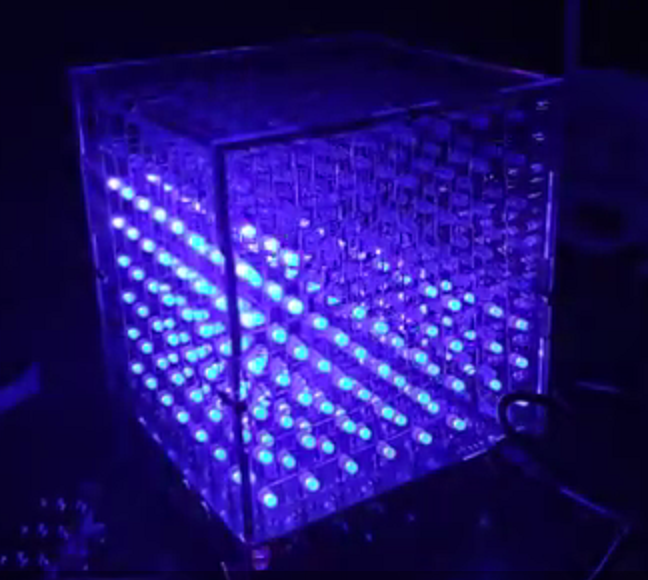
\includegraphics[scale=0.6]{pic/show1.png}
    \\\small{展示效果图}
\end{center}
展示视频链接如下:

\section{文件说明}
本项目文件说明如下表:\footnote{完成者中带*对应的文件,参考了\url{https://github.com/Ugon/fpga-fft-equalizer}或直接使用Altera中的PLL,并非完全独立实现。}
\begin{table}[h]
    \centering
    \resizebox{\textwidth}{!}{
    \begin{tabular}{|l|l|l|}
    \hline
    文件名                           & 功能                                       & 完成者 \\ \hline
    AN831.vhd                     & 读入AN831模块的输出,进行FFT                & 任一  \\ \hline
    audio\_processor.vhd          & 由时域数字信号做FFT得到频域数字信号                      & 任一*  \\ \hline
    dsp\_slave\_reader.vhd        & 将串行的ADCDAT以样本点为单位转为并行                    & 任一*  \\ \hline
    fft\_dif.vhd                  & 递归实现FFT                                  & 任一*  \\ \hline
    fft\_input\_deserializer.vhd  & 为FFT准备时域信号                               & 任一*  \\ \hline
    fft\_twiddle\_factors\_64.vhd & FFT计算中用到的旋转因子                            & 任一*  \\ \hline
    fft\_utils.vhd                & FFT计算中用到的函数                              & 任一*  \\ \hline
    i2c\_clk\_prescaler.vhd       & 时钟分频,由50MHz转换为100kHz                     & 任一* \\ \hline
    i2c\_master\_writer.vhd       & 配置WM8731芯片寄存器                            & 任一*  \\ \hline
    mTransmitter.vhd              &                                          & 潘传宇 \\ \hline
    mTXD.vhd                      &                                          & 潘传宇 \\ \hline
    mw8731\_controller.vhd        & 处理ADCDAT,配置WM8731芯片寄存器                & 任一*  \\ \hline
    mypll.vhd                     & 时钟分频,由100MHz转换为50MHz                     & 任一*  \\ \hline
    top.vhd                       & 顶层模块,连接音频处理和灯光信息传输模块 & 任一、潘传宇  \\ \hline
    trans\_pkg.vhd                &                                          & 潘传宇 \\ \hline
    \end{tabular}}
    \caption{项目文件说明}
    \end{table}
\section{总体设计}
\subsection{整体框架}
\paragraph{}本项目设计的整体框架如Figure\eqref{structure}所示。 
整个工程的输入为3.5mm的音频线,输入的是模拟信号。经过AN831模块中的WM8731芯片的模数转换,
得到24位的数字信号。数字信号输入FPGA后,由FPGA做FFT和数据的打包处理,由RX/TX串口将灯光信号
发送给光立方,光立方产生显示效果。


\begin{figure}[h]
    \centering
    \label{structure}
        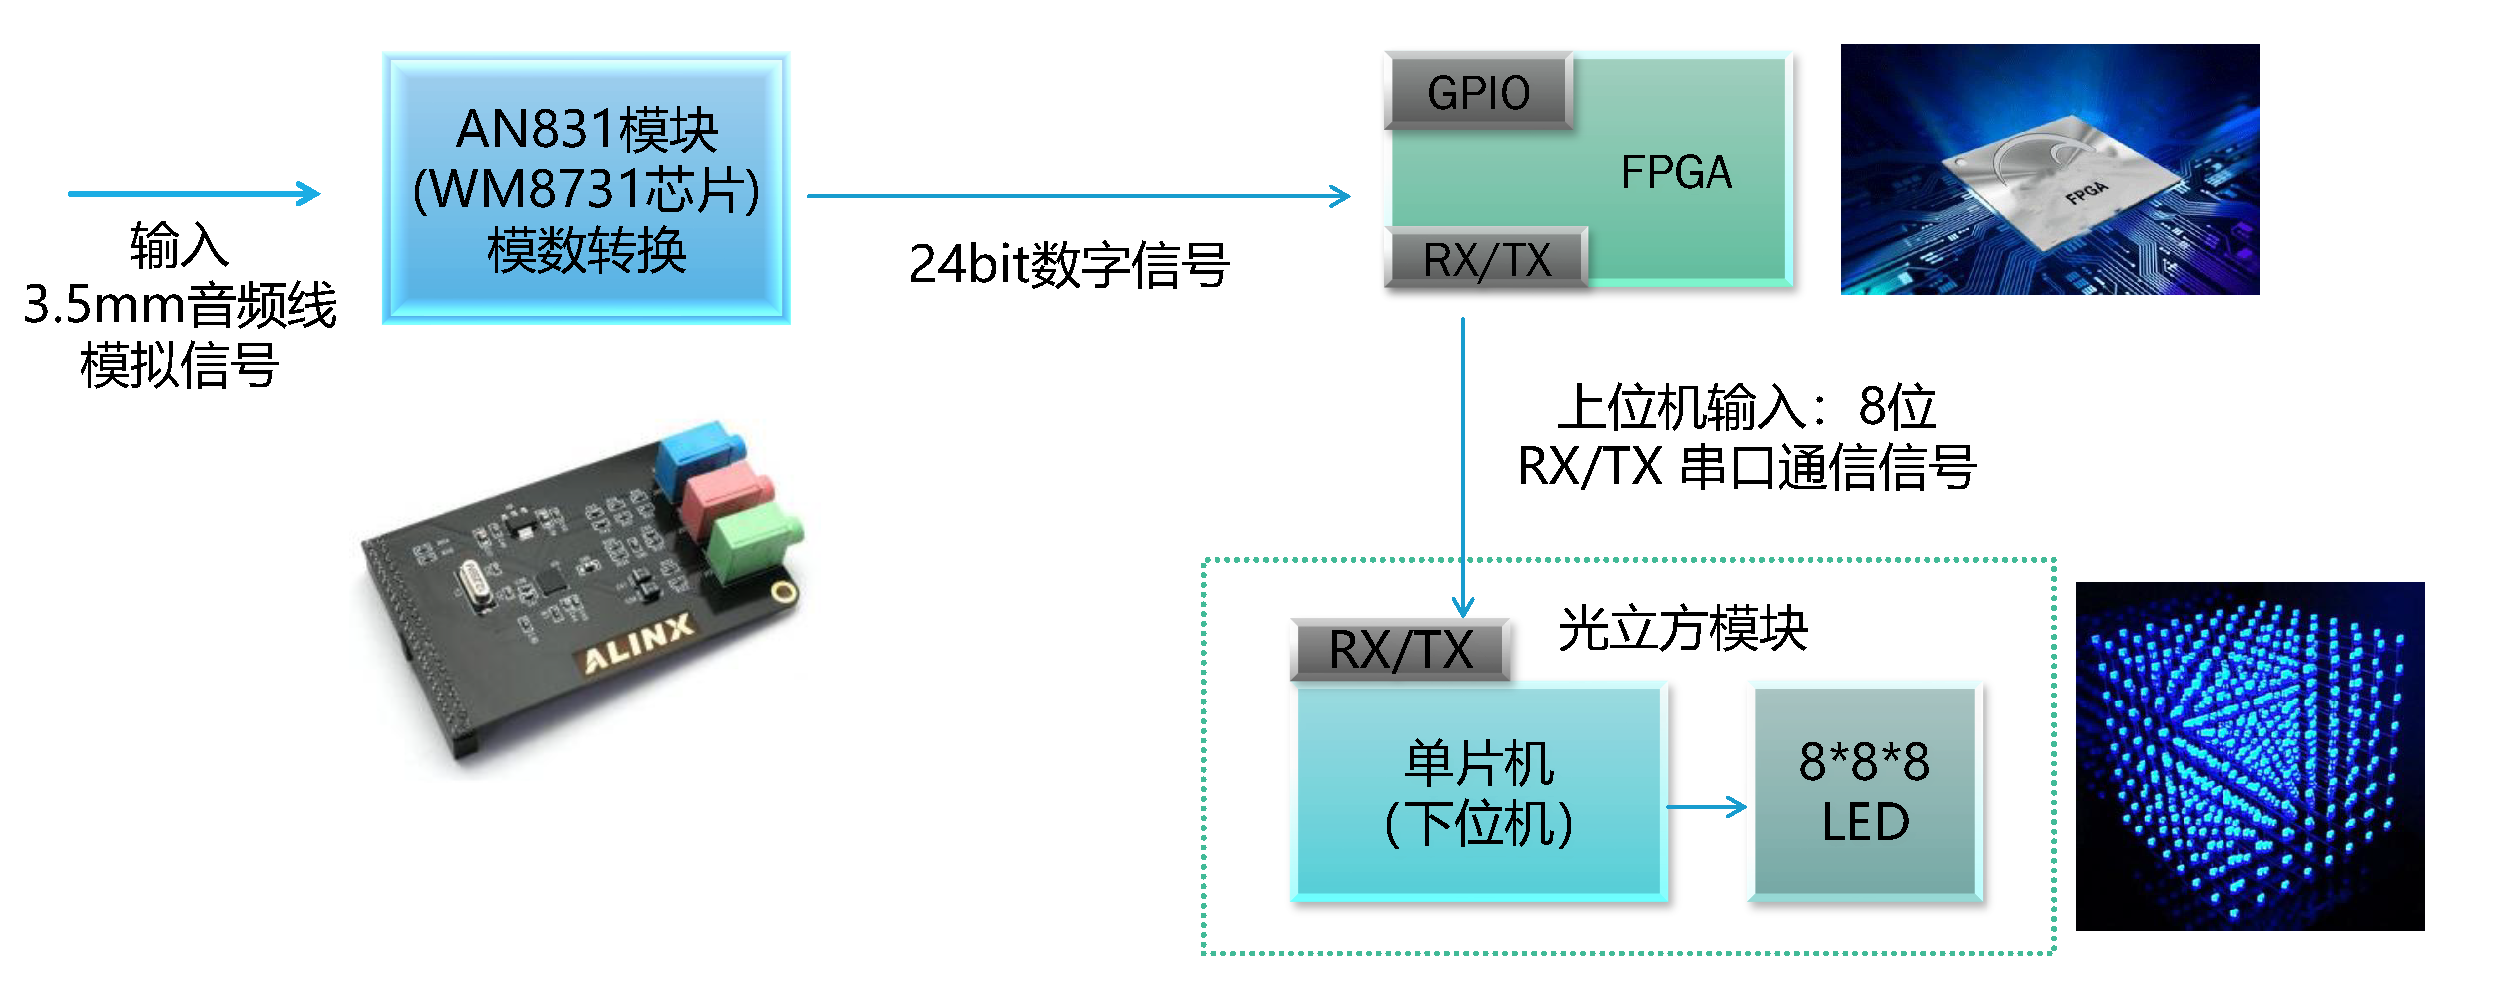
\includegraphics[width=0.8\textwidth]{./pic/structure.png}
        \caption{整体框架图}
\end{figure}


\subsection{FPGA设计概要}
\paragraph{}
FPGA设计概要如Figure\eqref{Design}所示。在FPGA中,我们首先接收了AN831模块输出的时域数字串行信号,并将其转为并行,
之后进行FFT,得到频域信号,由频域信号再转为灯光信息。
接着将灯光信息进行存储和整合,最后由UART串口输出给光立方。

\begin{figure}[h]
    \centering
    \label{Design}
        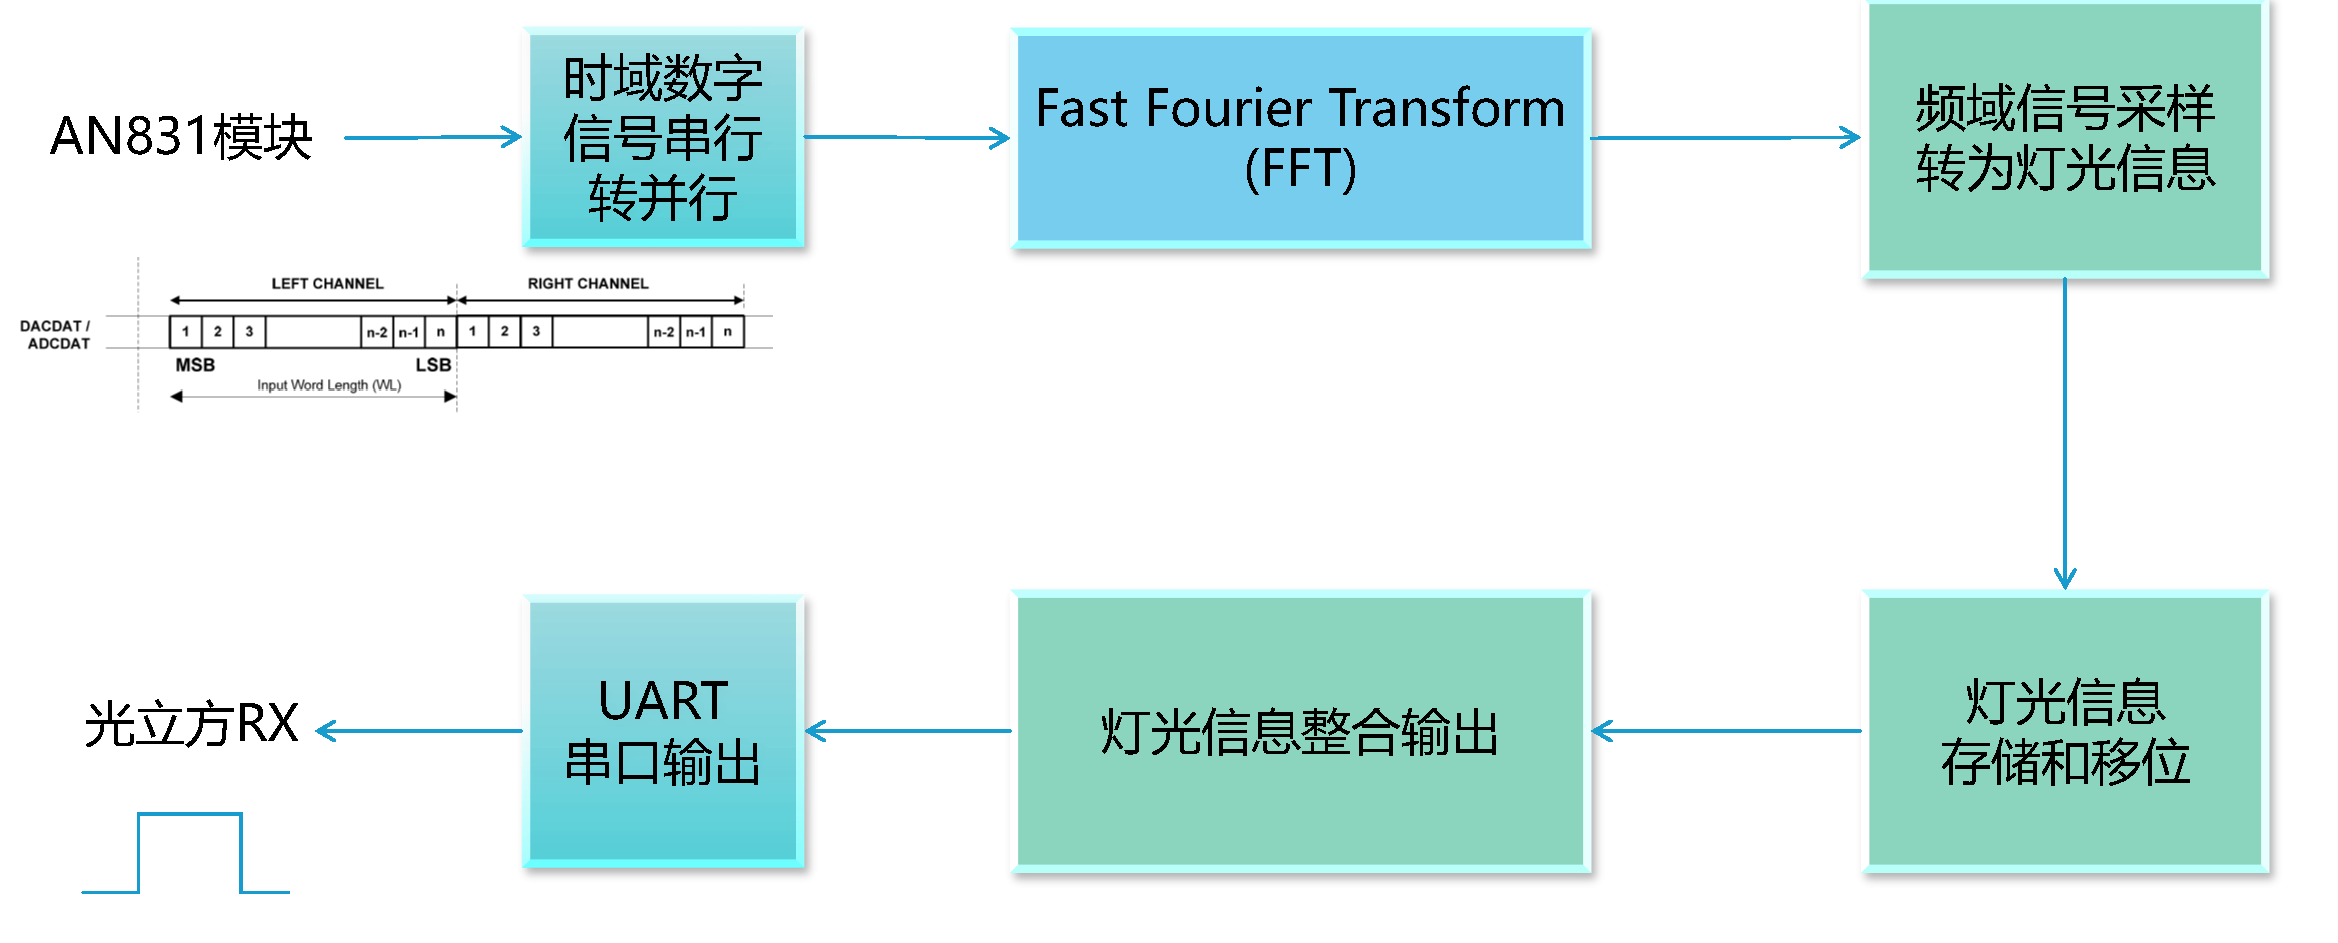
\includegraphics[width=0.8\textwidth]{./pic/Design.png}
        \caption{FPGA设计概要图}
\end{figure}


\subsection{光立方工作原理}
\paragraph{}
光立方的工作原理示意如Figure\eqref{cube}所示。
光立方是三维的显示,三个维度分别是时间、频率和强度。
随着时间的推移,光立方的显示沿着时间轴队列式逐层后移。
从频率-强度平面来看,光立方的8列分别代表8个频率分量的强度。
亮灯多的列对应的频率分量强度大,亮灯少的列对应的频率分量强度小。
同时,音量的大小也与强度有一定正相关关系,音量大则强度大,音量小则强度小。

\begin{figure}[h]
    \centering
    \label{cube}
        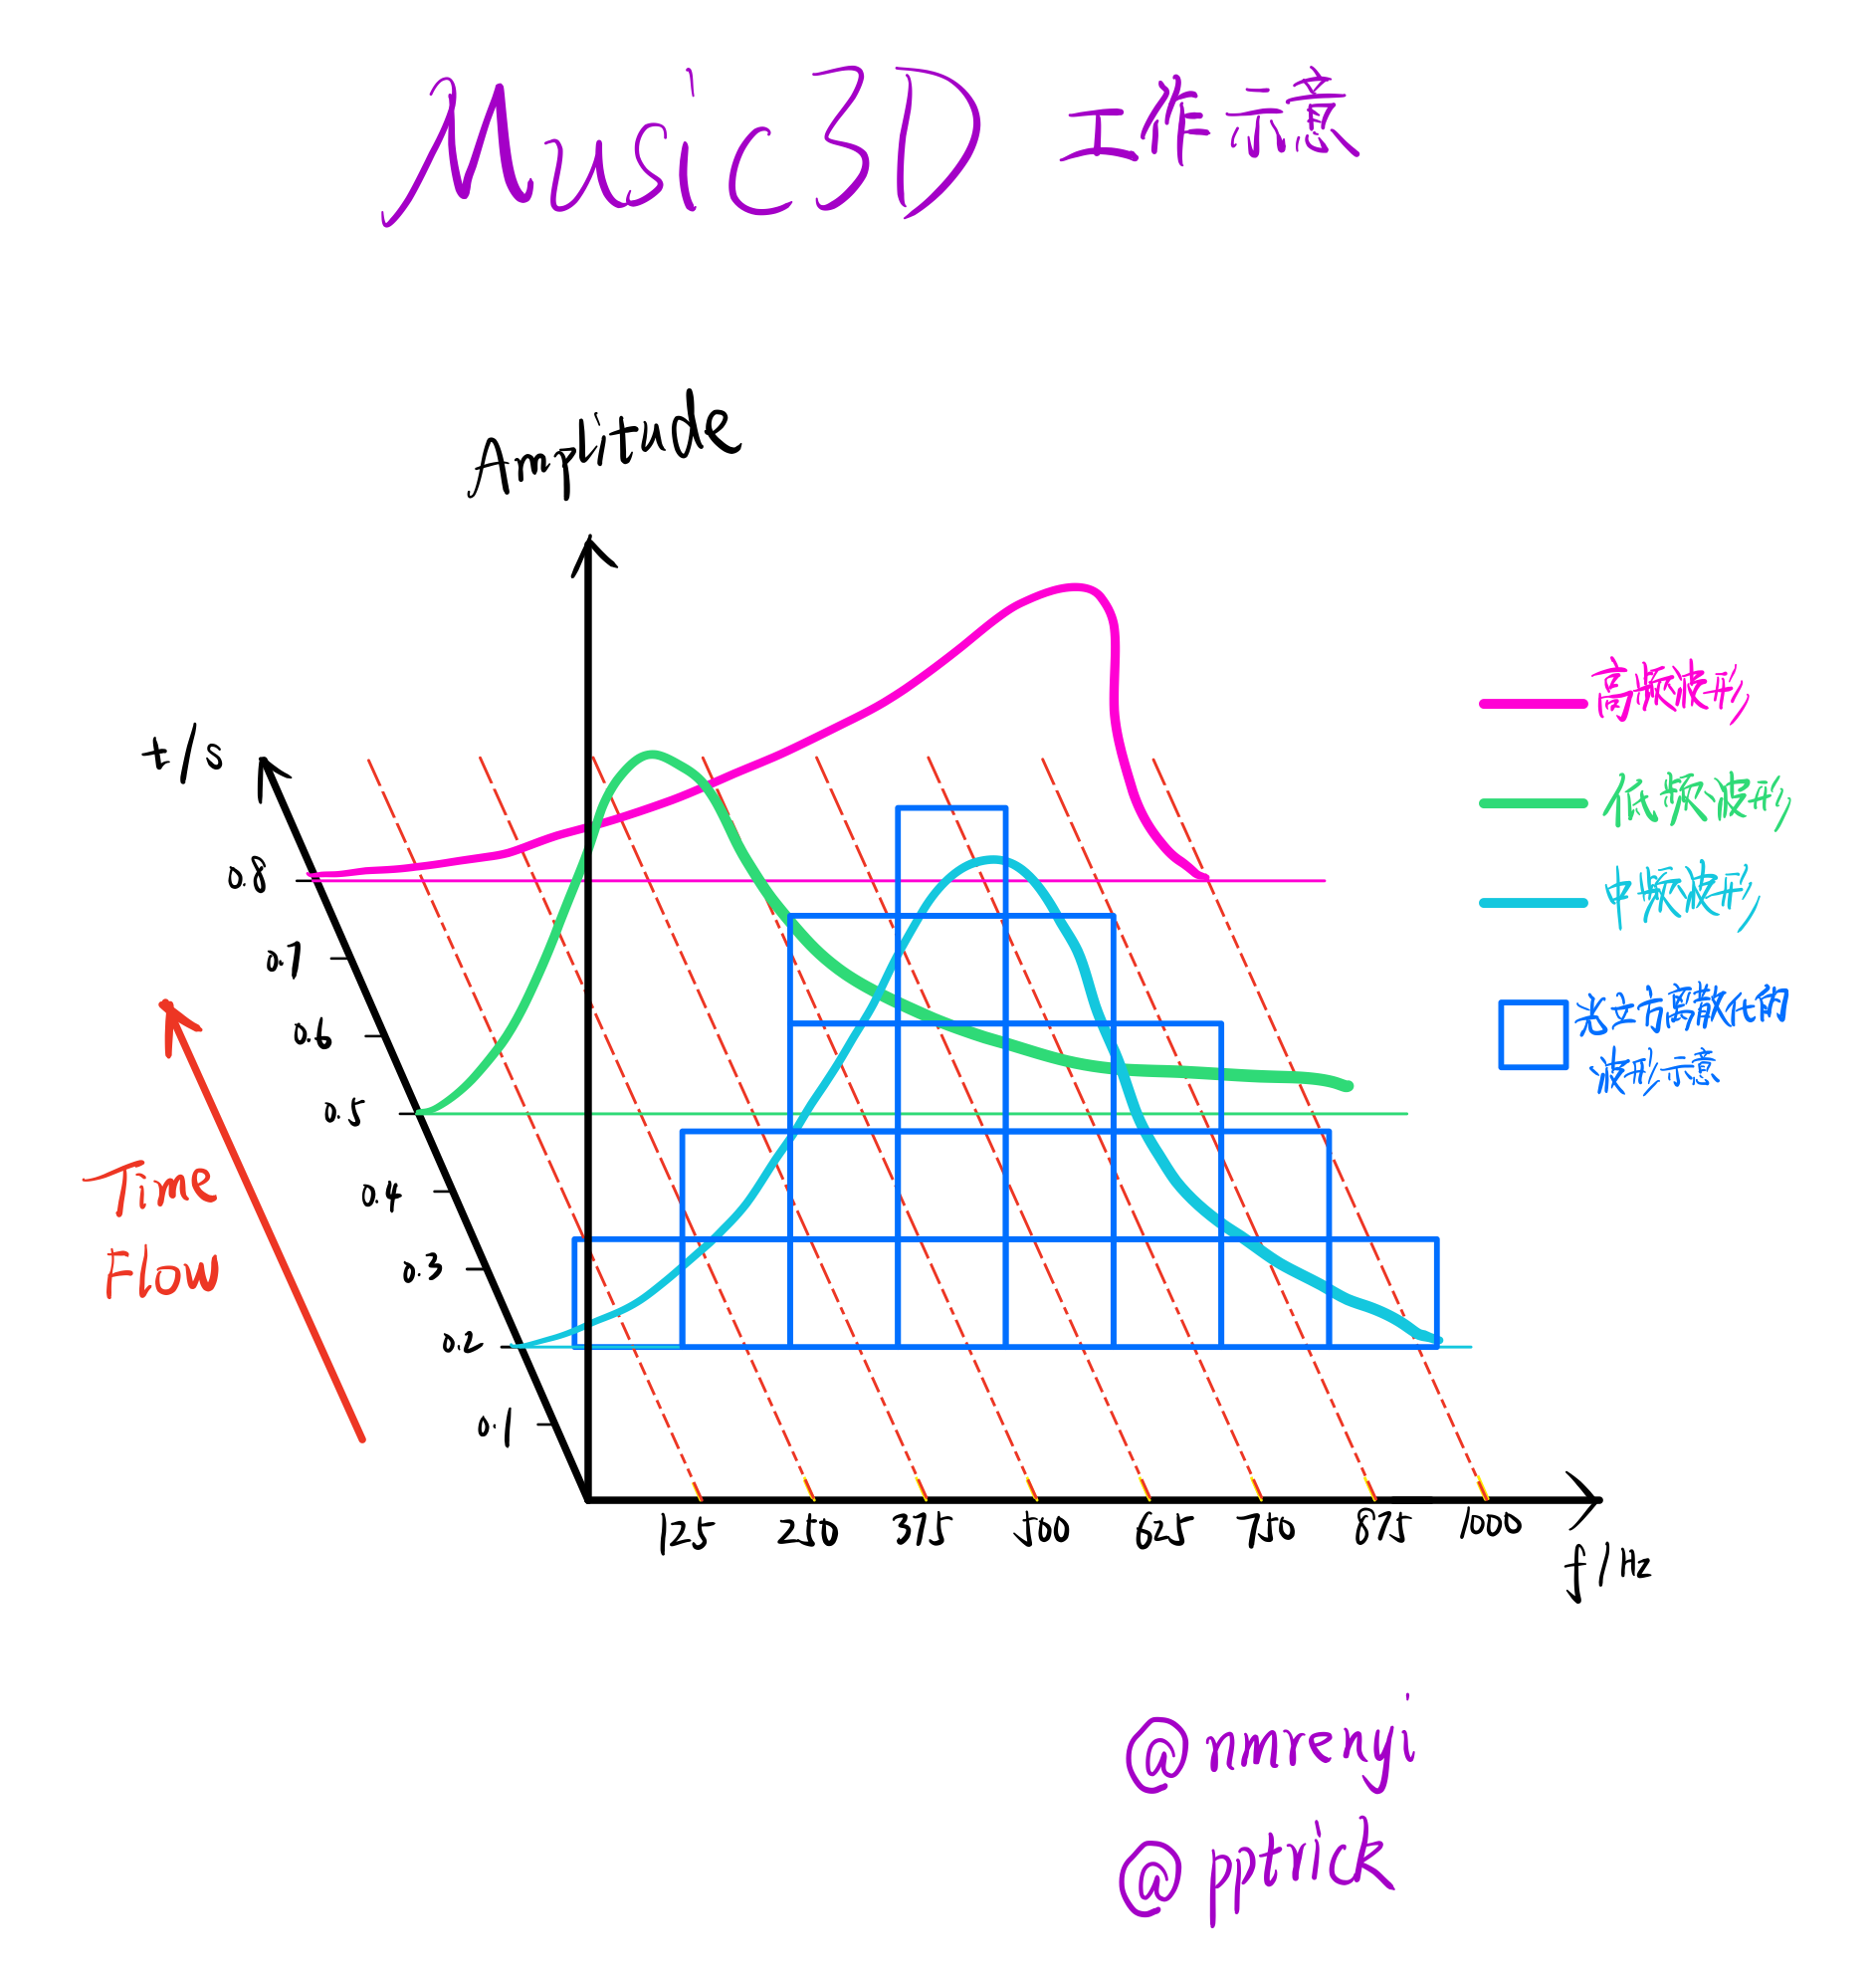
\includegraphics[width=0.8\textwidth]{./pic/ProjectWork.png}
        \caption{光立方工作原理示意图}
\end{figure}


\section{关键技术分析}
\subsection{Fast Fourier Transformation}
\paragraph{}为了从时域信号中提取频域信息,我们需要使用快速傅里叶变换(FFT)。在本代码中,我们配置WM8731芯片的采样频率为8KHz, 进行64点的FFT,得到了125Hz, 250Hz, 375Hz, 500Hz, 625Hz, 750Hz, 875Hz, 1000Hz
这8个频率处的频谱分量,正好对应光立方每一帧的8列灯光信息。为了节约计算成本,我们在进行FFT时,通过定点数的方式,提前储存了旋转因子。

\subsection{串口协议通信}
\paragraph{}通过UART串口传送串行信号,可以将设计好的灯光信息传给光立方模块上的单片机(相当于下位机),并由单片机控制灯的亮灭。
每一时刻的灯光信号由65个8位(并行)逻辑向量构成,需要将这些8位并行数据转化为串行的01输出,因此需要编写串口协议通信模块。该模块基于状态机
实现,通过不同状态表示当前输出处于起始位、数据位、校验位还是停止位,并通过计数方法使之适应相应的波特率。

\subsection{灯光信息整合输出}
\paragraph{}灯光信息采用“队列”结构存储,即每一时刻由采样模块收集频域信息并转化为灯光信息,将该灯光信息传入“队尾”,然后将“队顶”信息弹出。
\paragraph{}每次传给光立方的数据是65个8位逻辑向量,它是由1个“起始位”和64个“数据位”构成的;在传输时需要依次将这些8位逻辑向量传给“串口通信模块”。实现这一功能的难点在于与频域采样频率和串口波特率之间相适配。
此模块同样基于状态机实现,用不同状态判断当前输出处于起始位、数据位还是停止位;同时由于采样频率远小于波特率,可以通过计数方法将灯光信息输送频率调整到一个较为恰当的值。



\section{程序注释}
\section{波形仿真结果说明}
\section{遇到问题与解决方法}
\subsection{FPGA逻辑资源不足}
\paragraph{}在最初的项目调试中,我们希望做到的是采样频率48kHz的1024点FFT。这样做存在的问题是,
由于FFT涉及到大量的乘法,导致板子的逻辑资源严重不足。

因此我们从两方面进行改进,一方面是降低FFT点数,从1024点降低到64点,使得计算复杂度降低,同时我们也降采样频率
由48kHz降低到8kHz,从而保证FFT得到的每两点之间的频率差不会过大。另一方面,我们降低了旋转因子定点数的位数,从
原项目的16bit旋转因子降低到14bit旋转因子,进一步降低了计算的复杂度。通过这两方面的改进,我们成功实现了采样频率为8kHz下,64点的FFT.

其他可能的改进思路还有降低采样深度(即bits per sample). 这样做的原理与降低旋转因子的位数相似,都能够降低FFT中乘法的资源使用。
但由于本项目使用的是WM8731的DSP模式传输数据,在DSP模式下WM8731模块仅支持24bit的采样深度,因此我们最终没有采用这种优化方案。此外,也可以
考虑从FFT的算法本身进行改进,例如利用移位代替乘除法等方法,降低硬件逻辑资源使用率。

\subsection{时序问题}
在编译时,我曾遇到Critical Warning(332148): Timing requirements not met. 这样的问题。
经过与助教讨论,我意识到这是时序出现了问题。
经过对项目中使用的时钟加入限制后,再次编译基本解决了这个问题。

\section{实验总结}

\end{document}